\documentclass{report}
\usepackage[utf8]{inputenc}


\usepackage[a4paper, total={6in, 8in}]{geometry}


\title{Entwiklung Algorithmus Obere Halswirbelsäule}
\author{Lukas Hörnig}
\date{Oktober 2017}

\usepackage[square,sort,comma,numbers]{natbib}
\usepackage{graphicx}
\usepackage[hidelinks]{hyperref}
\usepackage{gensymb}

\begin{document}
\section{Klinische Instabilität}
\begin{figure}[h]
        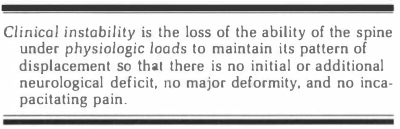
\includegraphics[width=8cm]{Instability.png}
\end{figure}

\section{Auswahl der Werte}
\subsection{Atlanto-occipitale Dislokation}
\paragraph{Distraktion, Trankslation}
% Doppelte Bewertung von AOD durch CS/CG und BDI?
% Werte und Studien zu BAI
Bevorzugung des Basion-Dens-Inteval (BDI) und Basion-posterior axial line Interval (BAI) \cite{WHOLEY1958,Harris1994,Harris1994a} über den Methoden Power's Ratio \cite{Powers1979} und X-Lines \cite{Lee1987}, durch Überlegenheit in Sensitivität, Spezifität, positiv prädiktivem und negativ prädiktivem Wert sowie in der Anwendbarkeit durch Lesbarkeit und Simpliziät. \cite{Deliganis2000,Fisher2001,Harris1994,Dziurzynski2005,Radcliff2010,Chang2009,Chaput2011,Bono2007}

\subsection{Atlantoaxiale Dislokation}

\section{Harris Measurements}
\subsection{Definiton}
\paragraph{Basion-Dens-Interval}

\begin{figure}[h]
        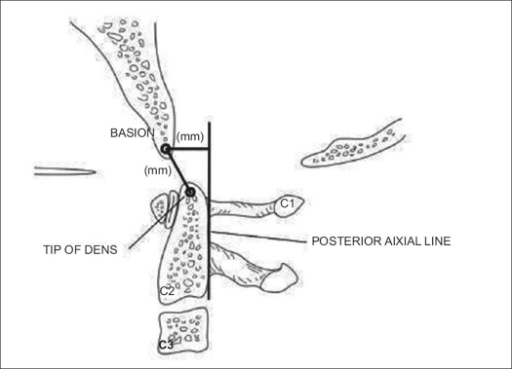
\includegraphics[width=8cm]{BDI.png}
\end{figure}

Länge der kürzesten Distanz zwischen dem Mittelpunkt des Basion und der Spitze des Dens in sagitaler Mittelininerekonstruktion in Millimetern.


\paragraph{Basion-posterior axial line - Interval}
Länge der kürzeste Distanz zwischen einer rechtwinkligen Linie vom Basion zu einer Verlängerung der Linie an der Hinterkante des vorderen Axisrings in sagitaler Mittelininerekonstruktion in Milimetern.

\subsection{Statistik}
Das BDI zeigt über die Altersgruppen und Geschlechter keine nennenswerte Instabilität \cite{Chaput2011} und wurde schon bezüglich Normwerte und pathologischer Abweichung ausgiebig untersucht.
\cite{Radcliff2010,Radcliff2012,Chang2009,Harris1994,Harris1994a,Chaput2011,Rojas2007,Gonzalez2004,Gonzalez2004a,Dziurzynski2005,Bono2007}. 



\paragraph{Validität}
% Resultiert aus Dislokation Instabilität??
Sowohl für die Sensibilität als auch für die Spezifität bezüglich des BDI für Atlanto-occipitale Dislokation und daraus resultierender Instabilität zeigen sich eine hohe Güte \cite{Dziurzynski2005}.

\paragraph{Reliabiliät}
% Hier fehlen noch die genauen Berechnungsformen und Kappa werte PDF-Chapter 6
Der BDI zeigt sich sowohl bezüglich Intra- und Interobserver Reliabiliät eine sehr hohe Güte \cite{Chaput2011,Dziurzynski2005,Harris1994,Harris1994a}, welche durch stabile Verhältnisse und verbesserte Bildgebung, sowie deren Lesbarkeit, welche durch verlässliche Darstellung der benötigten anatomischen Landmarken garantiert werden \cite{Dziurzynski2005,Radcliff2010}.


\subsection{Patholgischer Wert}
% Auswertung Graphisch wie in \cite{Woods2017}
Ab einem BDI von über 10 mm und/oder einem BAI von mehr als 12 mm sollte von einer Instabilität durch Atlanto-occipitale Dislokation ausgegangen werden.


\subsection{Anwendbarkeit}
Die Anwendbarkeit wird bei Messung an CT-Bildgebung durch hochaufgelöste, überlagerungsfreie Darstellung für erfahrene Anwender der Technik sehr zuverlässig und in fast allen Fällen möglich gemacht \cite{Dziurzynski2005,Radcliff2010}. 


\section{LMI}
Das LMI zeigt über Altersgruppen und Geschlechter hinweg eine statistisch signifiktante Instabilität \cite{Chaput2011}



\section{Lateral Mass Displacement}
\bibliography{../literatur}
\bibliographystyle{dinat}
\end{document}
